\documentclass{../cssheet}

%--------------------------------------------------------------------------------------------------------------
% Basic meta data
%--------------------------------------------------------------------------------------------------------------

\title{Sätze am Kreis}
\author{Prof. Dr. Christian Spannagel}
\date{\today}
\setsubject{Aufgabenblatt Geometrie}
\setkeywords{geometrie}
\setpdfmetadata


%--------------------------------------------------------------------------------------------------------------
% document
%--------------------------------------------------------------------------------------------------------------

\begin{document}

\printtitle

\textbf{Aufgabe 1 (Satz des Thales):}  Der Satz des Thales lautet: Verbindet man zwei Endpunkte $A$ und $B$ eines Kreisdurchmessers mit einem weiteren Punkt $C$ auf der Kreislinie, so entsteht bei $C$ ein rechter Winkel.

Beweist den Satz des Thales.

\textbf{Aufgabe 2 (Satz des Thales: Umkehrung):} Formuliert die Umkehrung des Satzes von Thales und beweist sie.

\textbf{Aufgabe 3 (Umfangswinkel und Mittelpunktswinkel):} Gegeben sei ein Kreis mit Mittelpunkt $M$, eine Sehne $\overline{AB}$ und ein Punkt $C$ auf der Kreislinie. 
\begin{center}
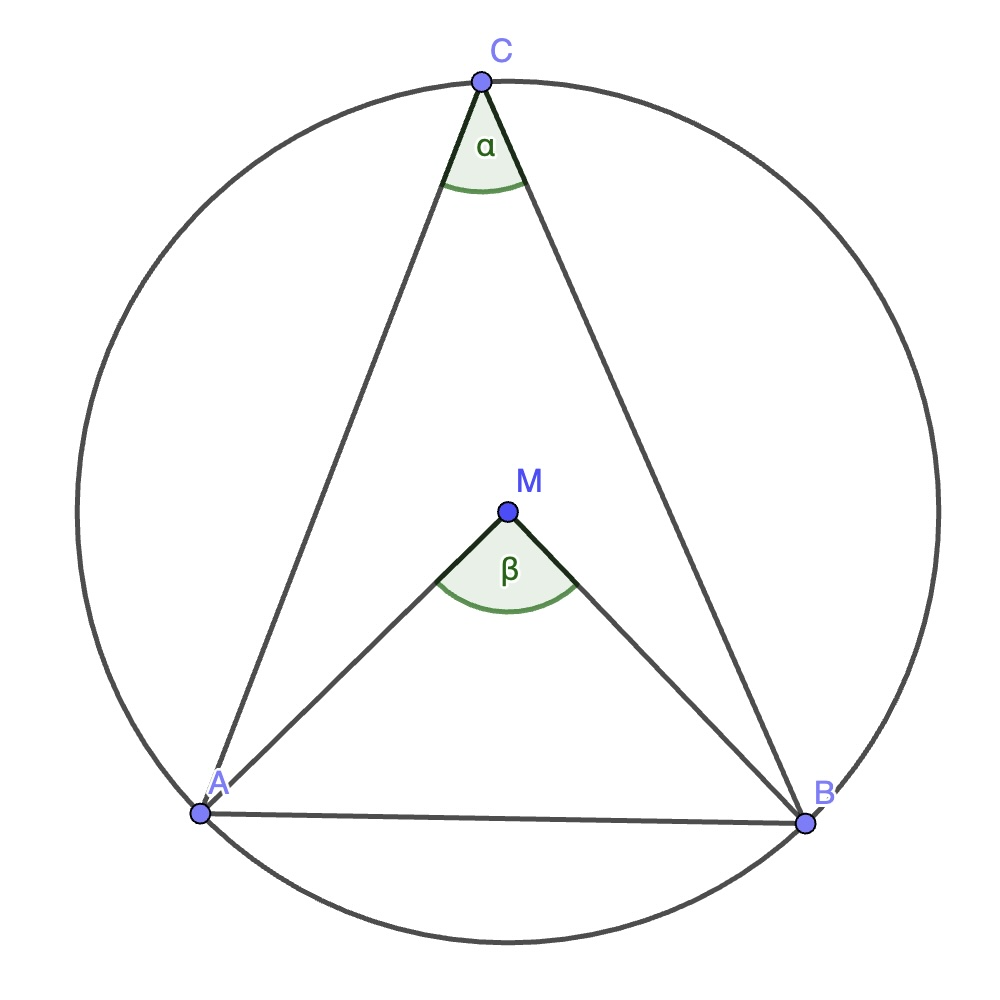
\includegraphics[width=8cm]{umfangswinkel.png}
\end{center}
Zu zeigen ist: Der Umfangswinkel $\alpha$ ist halb so groß wie der Mittelpunktswinkel $\beta$. Konstruiert zunächst die Situation in Geogebra und vergewissert euch durch Ausprobieren. Beweist die Aussage anschließend.

\textbf{Aufgabe 4 (Umfangswinkelsatz):}  Beweist, dass alle Umfangswinkel über einer Kreissehne gleich groß sind.

%\newpage
\vspace*{10mm}
\printlicense

\printsocials


%\pagestyle{docstyle}
\end{document}
